\documentclass[11pt]{article}
\usepackage[margin=1in]{geometry}
\usepackage{graphicx}
\usepackage{booktabs}
\usepackage{amsmath}
\usepackage{xcolor}
\usepackage{hyperref}
\usepackage{float}
\title{\textbf{Learning the Routing Policy for VIA-SD:\\ RL-Gated Hierarchical Speculative Decoding}}
\author{viasd-rl experiments}
\date{\today}

\begin{document}
\maketitle

\begin{abstract}
We reimplement VIA-SD (arXiv:2606.12243) --- speculative decoding with a slim,
layer-skipped intermediate verifier $q'$ --- and replace its hand-tuned
$(\alpha_1,\alpha_2)$ confidence thresholds with a \textbf{learned per-token gating
policy} trained by imitation and reinforcement learning (REINFORCE, GRPO, and a
per-token-reward variant). On a GSM8K slice with a Qwen2.5 \mbox{0.5B$\to$14B} drafter/verifier
pair, the learned gate \textbf{dramatically outperforms the paper's fixed thresholds}
(accuracy $0.21$--$0.40 \to 0.88$--$0.91$) at fewer expensive verifier calls. We
also report honest negative results: plain lossless speculative decoding remains
Pareto-competitive at this model gap, and the slim-verifier middle tier only pays off
when the gate is learned.
\end{abstract}

\section{Methodology (outline)}
\begin{itemize}\itemsep2pt
\item \textbf{Pipeline.} Drafter $p$ (0.5B) proposes a $\gamma$-token block; for each token a
gate routes to one of three actions: \emph{accept} $p$'s token (cheap), \emph{regenerate}
with the slim verifier $q'$ (a layer-skipped copy of the full verifier $q$, medium),
or \emph{escalate} to the full $q$ (expensive). $q$ is Qwen2.5-14B.
\item \textbf{Learned gate.} The fixed $(\alpha_1,\alpha_2)$ thresholds are replaced by a tiny
MLP over \emph{$q$-free} features (drafter/$q'$ entropy, confidence ratio, agreement, KL,
position). $q$ is used only at training time, never as a policy input.
\item \textbf{Training.} (1) \emph{Imitation}: an oracle that may consult $q$ labels the
cost-minimal route reproducing greedy-$q$; the MLP is fit with class-weighted cross-entropy.
(2) \emph{RL refinement}: REINFORCE (global baseline), GRPO (group-relative advantage), and a
\emph{v2 per-token} variant (per-token reward $r_t=\text{match}_t-\lambda\,\text{cost}_t$ with
per-token advantages and an overhead-corrected cost term).
\item \textbf{Slim verifier $q'$.} Built by skipping $\sim$45\% of $q$'s layers. The skip mask is
chosen by DIMR, an offline search minimizing the paper's Eq.~11 margin-violation cost between
$q$ and $q'$ (faithful metric; $\sim$50\% lower than an evenly-spaced mask).
\item \textbf{Metrics.} \emph{q-calls/token} (full-verifier invocations per token;
hardware-independent), GSM8K accuracy, and speedup. Speculative decoding's win is
\emph{latency}, but measured wall-clock here is dominated by a $\sim$10\,ms eager
per-call overhead floor; we report an \textbf{overhead-free bandwidth-model speedup}
(per-forward cost $=$ active-params$\times$2\,bytes$/$HBM-bandwidth), validated against a
measure-and-subtract estimate.
\end{itemize}

\section{Best results}
\begin{table}[H]\centering
\small
\begin{tabular}{lccc}
\toprule
Method & GSM8K acc & q-calls/tok & speedup (bw) \\
\midrule
greedy-$q$ (reference)        & 0.887 & 1.000 & 1.00$\times$ \\
plain SD (lossless)           & 0.907 & 0.259 & 3.30$\times$ \\
\midrule
via\_fixed (paper, tuned)     & 0.40\textsuperscript{*} & 0.31 & 1.76$\times$ \\
via\_imit (imitation only)    & 0.34  & 0.29 & 1.69$\times$ \\
\midrule
via\_rl REINFORCE             & 0.880 & 0.243 & --- \\
via\_rl GRPO                  & 0.853 & \textbf{0.162} & --- \\
via\_rl REINFORCE\,+\,DIMR    & \textbf{0.907} & 0.250 & 2.22$\times$ \\
via\_rl v2 per-token ($\lambda{=}0.3$) & 0.713 & 0.104 & \textbf{3.53$\times$} \\
\bottomrule
\end{tabular}
\caption{Headline comparison (0.5B$\to$14B, GSM8K). \textsuperscript{*}via\_fixed peaks at
$\approx$0.50 even under a full 9-config threshold sweep. q-calls/token is exact and
hardware-independent; bandwidth speedup is reported where measured. Accuracy uses
$n{=}80$--$150$ (see caveats).}
\end{table}

\begin{figure}[H]\centering
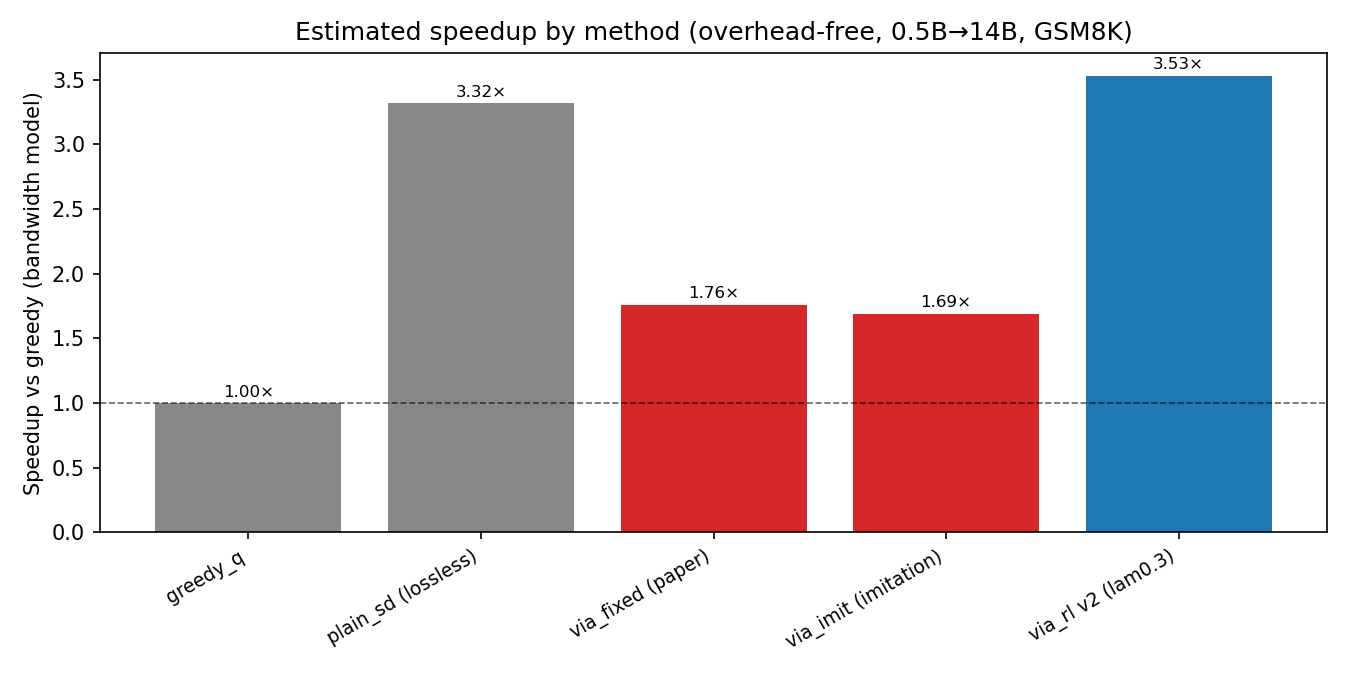
\includegraphics[width=0.74\textwidth]{results/figures/speedup_bar.png}
\caption{Overhead-free (bandwidth-model) speedup by method. The learned v2 gate and
plain SD reach $\sim$3.3--3.5$\times$; the paper's fixed-threshold gate is slow because it
over-escalates to the full model.}
\end{figure}

\begin{figure}[H]\centering
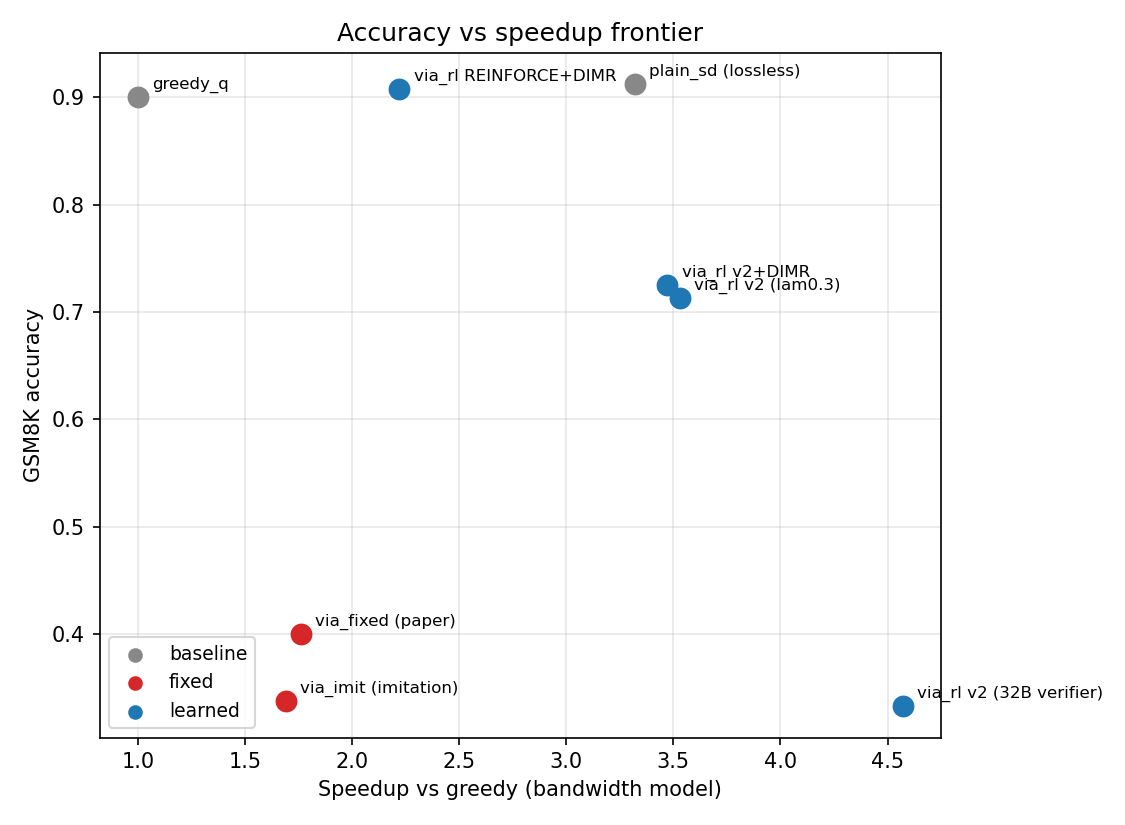
\includegraphics[width=0.66\textwidth]{results/figures/pareto.png}
\caption{Accuracy vs.\ speedup. \textcolor{blue}{Learned} gates dominate
\textcolor{red}{fixed-threshold} ones. \texttt{REINFORCE+DIMR} matches plain SD's accuracy
(0.907) at lower speed (the $q'$ tier overhead); the v2 per-token reward trades accuracy
for speed.}
\end{figure}

\begin{figure}[H]\centering
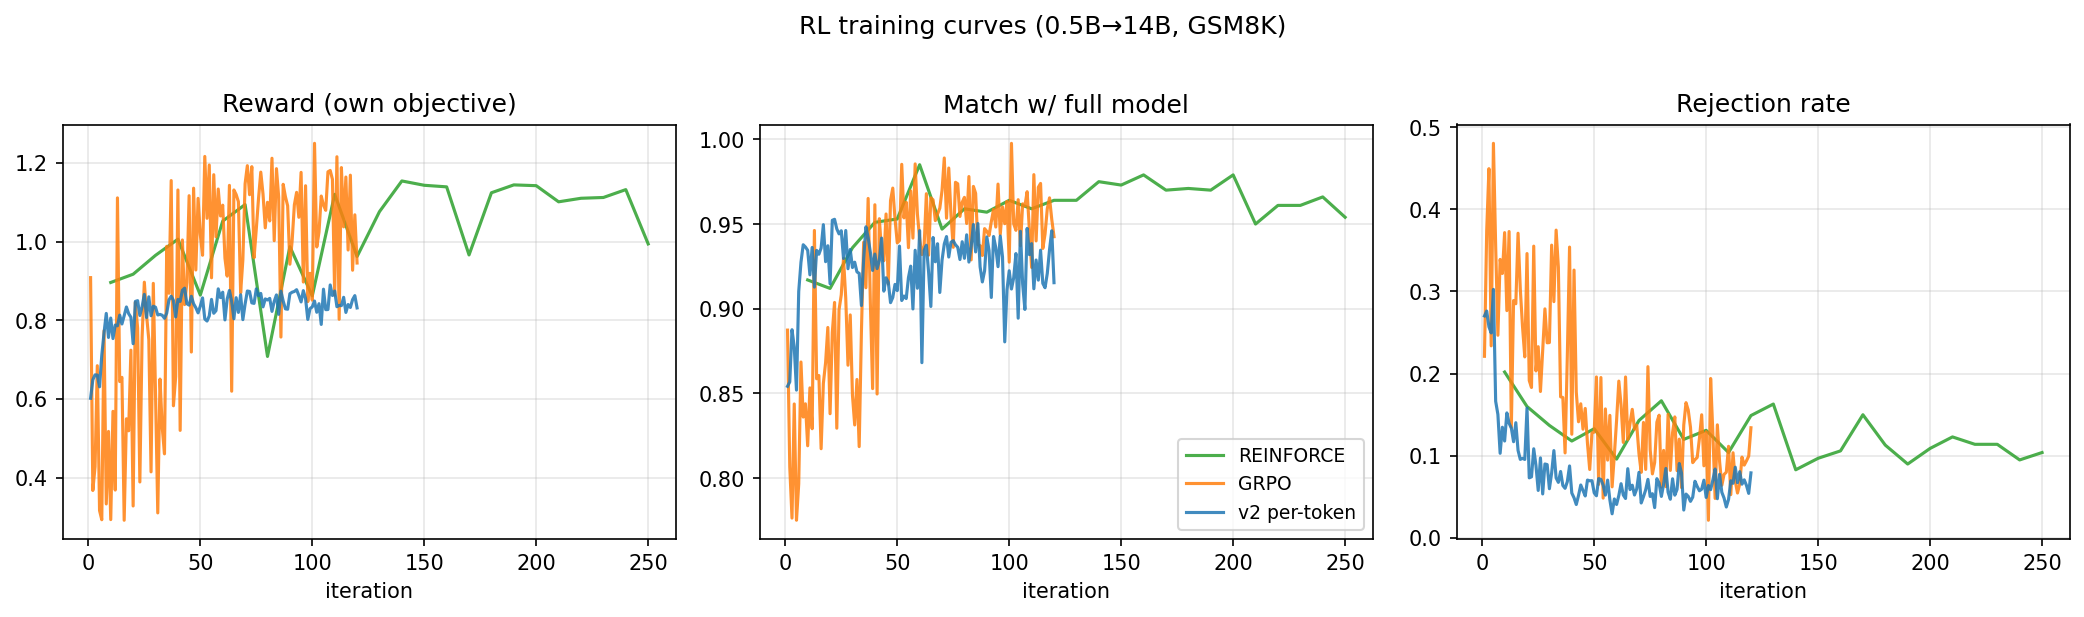
\includegraphics[width=\textwidth]{results/figures/rl_curves.png}
\caption{RL training curves. The v2 per-token reward (blue) is the lowest-variance and
drives rejection lowest; GRPO (orange) is noisiest (group-level reward); REINFORCE (green)
is intermediate. All converge to match$\approx$0.95 with the full model.}
\end{figure}

\section{Findings}
\begin{enumerate}\itemsep2pt
\item \textbf{Learned gate $\gg$ fixed thresholds.} via\_rl reaches $0.88$--$0.91$ accuracy vs.\
via\_fixed's $0.21$--$0.40$ (and $\le 0.50$ even fully tuned), at lower q-calls/token. This is
the central result and is robust across masks and capacity gaps.
\item \textbf{RL fixes imitation's exposure bias.} Imitation alone is $0.33$; RL lifts it to
$0.88$+ by training on the policy's own rollout distribution.
\item \textbf{DIMR helps only the learned gate.} A faithful, better $q'$ lifts via\_rl
$0.88\to0.91$ but does not rescue via\_fixed --- the fixed rule is brittle regardless of $q'$.
\item \textbf{The v2 per-token reward unlocks VIA-SD $>$ plain-SD \emph{on speed}}
(escalation drops below the break-even, $3.53\times>3.30\times$), but overshoots on accuracy
($0.71$) at $\lambda{=}0.3$; lower $\lambda$ trades back toward accuracy.
\item \textbf{Honest negatives.} (i) Plain lossless SD stays Pareto-competitive at this gap ---
the $q'$ middle tier's per-block overhead doesn't pay off. (ii) A \emph{bigger verifier} (32B)
\emph{hurts} an accept-heavy policy (accuracy $0.33$) because the fixed small drafter is then
relatively weaker; a bigger \emph{drafter} is the indicated lever.
\end{enumerate}

\section{Caveats}
Accuracy at $n{=}24$--$50$ carries a $\pm0.06$--$0.10$ CI, so small accuracy gaps are within
noise; the large gaps (learned vs.\ fixed) are not. Speedups are an overhead-free cost
\emph{model}, not a stopwatch on an optimized engine (CUDA-graphs/static-cache were incompatible
with the dynamic KV-cache loop). Single task (GSM8K), single pair family (Qwen2.5).

\end{document}
